Le crible d’Ératosthène est un moyen très simple de de trouver les nombres premiers en partant de 2. Mais il y a plusieurs inconvénients quant à l'utilisation de cet algorithme.

\subsubsection{Fonctionnement}

Le crible d’Ératosthène se décompose en deux phases :
\begin{itemize}
\item Une première phase d'initialisation qui consiste à remplir une liste commençant à 2 et finissant au nombre jusqu'au quel nous voulons chercher des nombres premiers.\\
\item La seconde phase consiste à passer la liste au crible pour isoler les nombres premiers : pour cela on parcourt la liste de nombres ; pour chaque nombre on reparcourt cette liste et on supprime tous ses multiples.\\
\end{itemize}
Une amélioration simple consiste à mettre 2 dans la liste lors de l'initialisation puis à entrer tous les nombres allant de 3 à la limite que l'on veut avec un pas de 2.


\subsubsection{Benchmark}

Le graphique suivant montre le temps que met l'algorithme pour calculer de 2 jusqu'à la limite.\\
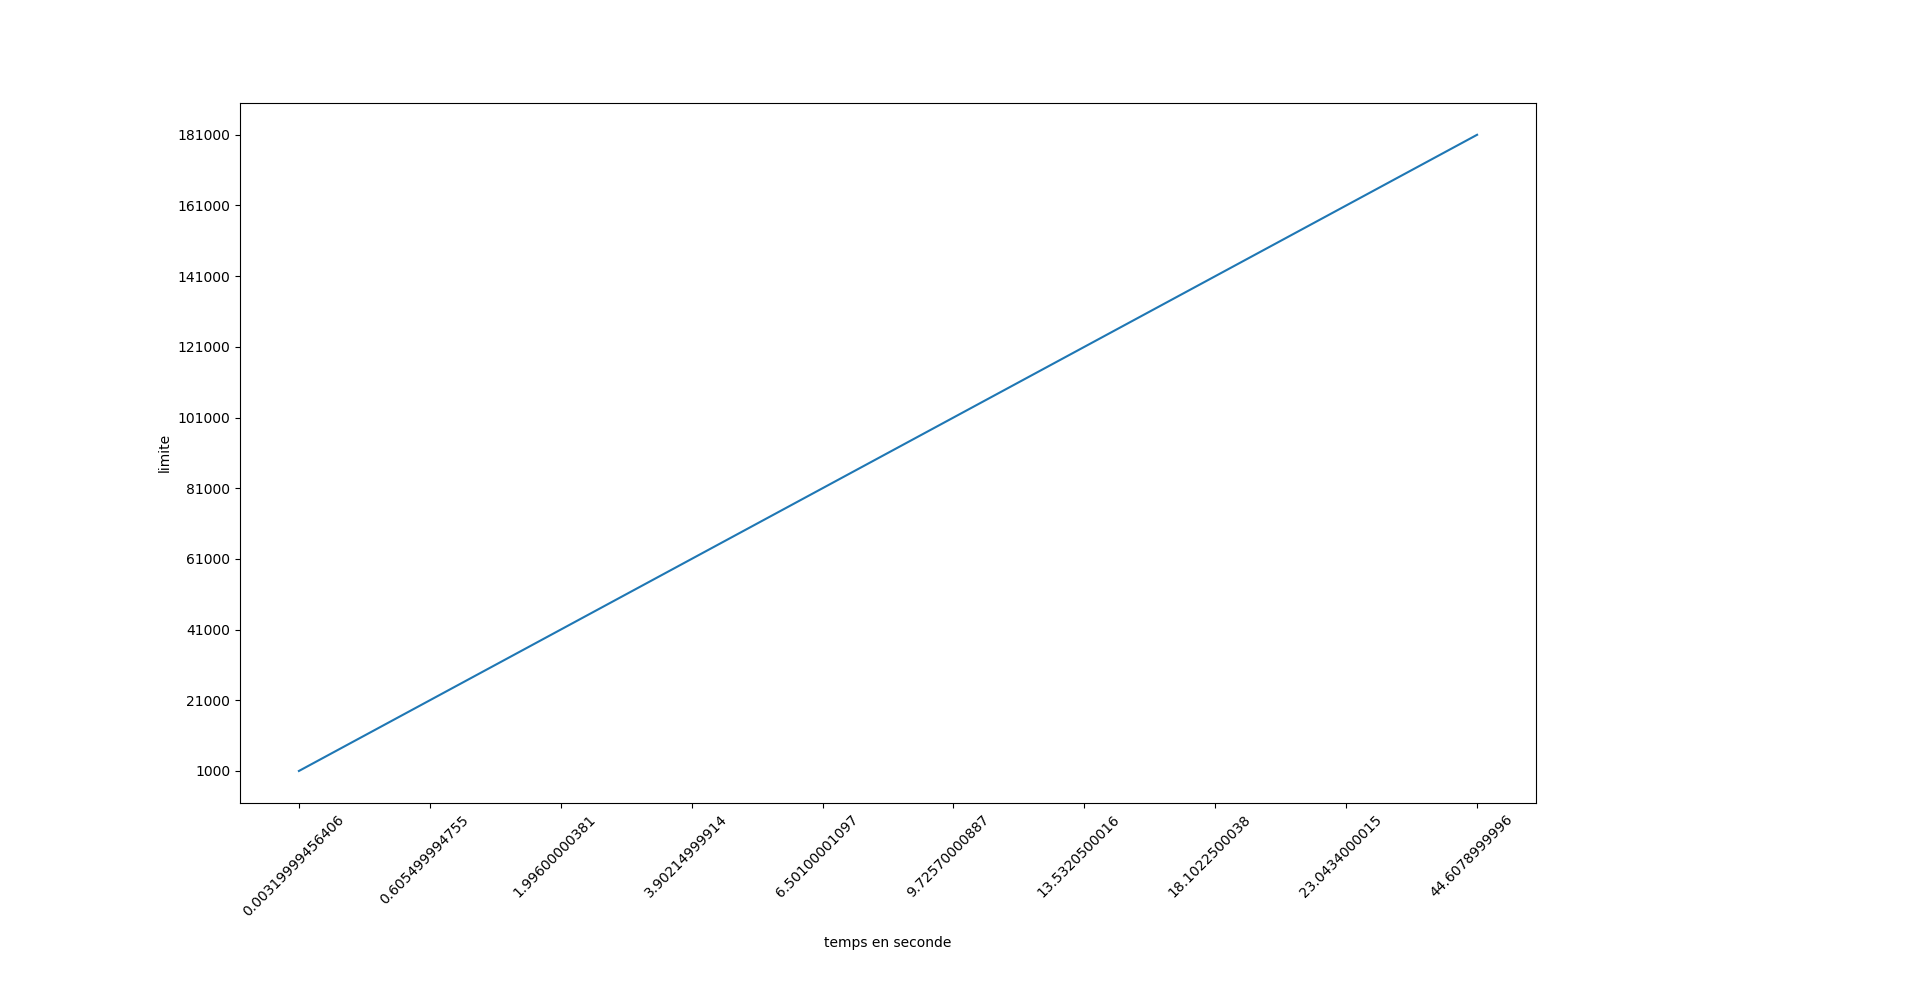
\includegraphics[scale=0.4]{images/erathostene1.png}
Comme on peut le voir, que alors que la limite augmente de façon linéaire ( de 20 000 en 20 000 ) alors que le temps lui augmente en $n^2$.\\
